\subsection{LoggerPro Curve Fitting.}

Let's start by noting that you can download LoggerPro to your own computer
if you would like. You should have received a notification about this on
I-Learn. If you wish to install LoggerPro, follow the announcement
instructions.

Once you have LoggerPro on your computer or on one of our lab computers, we
will use it for fitting a curve to our data just like we did last time in
Excel. Suppose you have already imported your data in Excel. It might look
like this:

\begin{figure}[h!]
	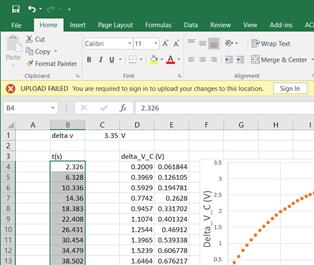
\includegraphics[width=2.6498in,height=2.2399in]{PH4CAX3C}
\end{figure}Now highlight a----- column (I
highlighted the time column) and select copy to copy the data to the
clipboard. Then open up LoggerPro. You will see a data area, a graph area,
and the toolbar.\begin{figure}[h!]
	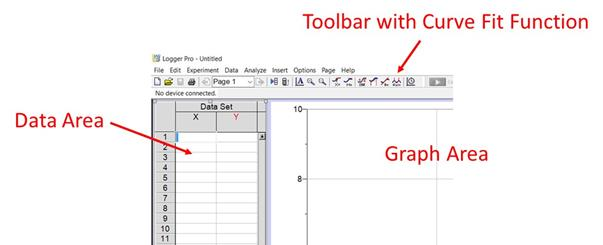
\includegraphics[width=5.0721in,height=2.0721in]{PH4CAX3D}
\end{figure}We want to past the data into a
column in LoggerPro. If you also selected the time data, paste it into the $%
x $-column in Logger Pro. \begin{figure}[h!]
	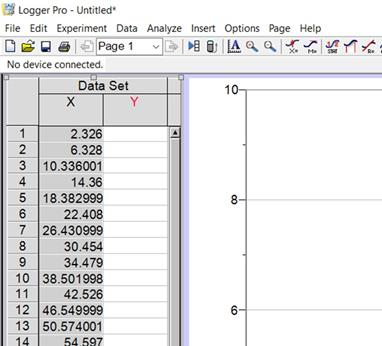
\includegraphics[width=3.2197in,height=2.9187in]{PH4CAX3E}
\end{figure}

Do the same for the voltage data. Paste it into the $y$-column. Once you do
this, the data will automatically be graphed. \begin{figure}[h!]
	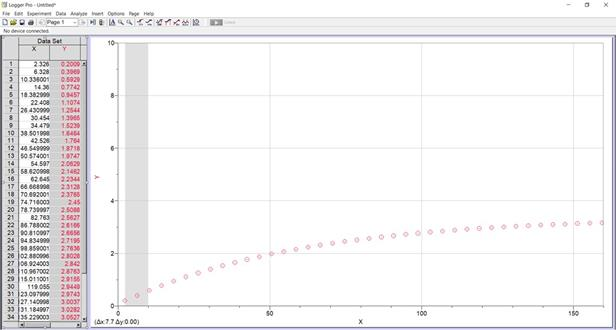
\includegraphics[width=5.1802in,height=%
	2.7838in]{PH4CAX3F}
\end{figure}We now want to fit a curve to
this data. The curve fit function can be accessed from the tool bar. It
looks like this: \begin{figure}[h!]
	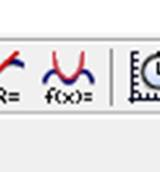
\includegraphics[width=1.3604in,height=1.4607in]{PH4CAX3G}
\end{figure}Click on the icon and a new
dialog will appear. \begin{figure}[h!]
	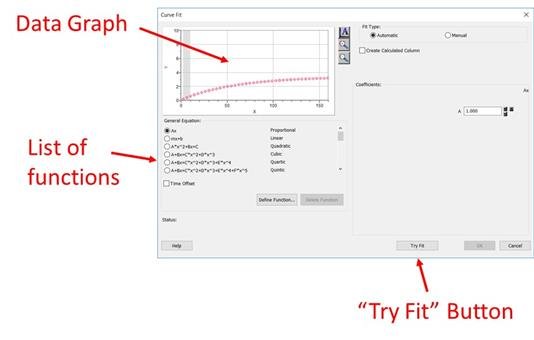
\includegraphics[width=4.4936in,height=2.8677in]{PH4CAX3H}
\end{figure}

It is tempting to try just any function to see if it fits. But the goal is
not to have a great fit. The goal is to see if our data fit the equation
from our capacitor model. 
\begin{equation*}
	\Delta V_{C}\left( t\right) =\Delta V_{\max }\left( 1-e^{-\frac{t}{\tau }%
	}\right)
\end{equation*}%
so we need to find this particular function. This is why I didn't suggest
using Excel. Excel does not have the equation we need in it's list.

\begin{figure}[h!]
	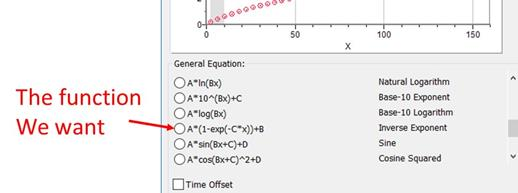
\includegraphics[width=3.2759in,height=1.2298in]{PH4CAX3I}
\end{figure}Of course we won't find a match
with our exact notation. The one we want is given as 
\begin{equation*}
	y=A\ast (1-\exp (-C\ast x))+B
\end{equation*}%
and now we have to match our variables with theirs. Let's compare the
equations. 
\begin{eqnarray*}
	y &=&A\ast (1-\exp (-C\ast x))+B \\
	\Delta V_{C}\left( t\right) &=&\Delta V_{\max }\left( 1-e^{-\frac{t}{\tau }%
	}\right) +0
\end{eqnarray*}%
We can see that 
\begin{equation*}
	\begin{tabular}{ll}
		Ours & Theirs \\ 
		$\Delta V_{\max }$ & $A$ \\ 
		$0$ & $B$ \\ 
		$\tau $ & $\frac{1}{\mathtt{C}}$%
	\end{tabular}%
\end{equation*}%
We can see this \begin{figure}[h!]
	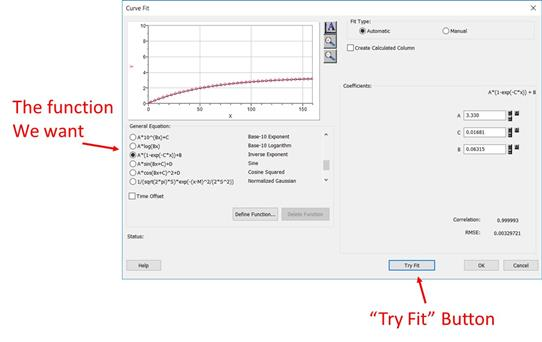
\includegraphics[width=4.561in,height=2.8842in]{PH4CAX3J}
\end{figure}

If the fit looks good, choose the \textquotedblleft OK\textquotedblright\
button. You get the graph back with the curve fit and a new little box. 
\begin{figure}[h!]
	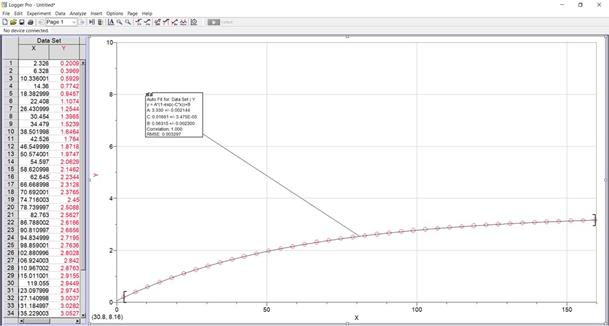
\includegraphics[width=5.1214in,height=2.751in]{PH4CAX3K}
\end{figure}The curve fit looks nice and that
is comforting. For my data, it looks like our capacitor model might be
correct, but we can't be sure until we add in error bars. Before we do that,
let's look at the new little box. \begin{figure}[h!]
	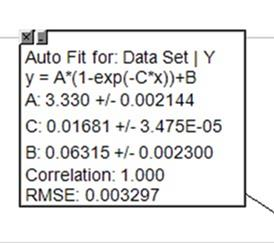
\includegraphics[width=2.3151in,height=2.0557in]{PH4CAX3L}
\end{figure}The box has our fit equation that
we chose and it has values for the fit parameters and their uncertainties.
We will need those later!

Let's add on the error bars now. Right click on the graph if you have a PC
or do the Mac equivalent if you have a Mac. A new dialog appears and in this
case choose \textquotedblleft Graph Options.\textquotedblright\ \begin{figure}[h!]
	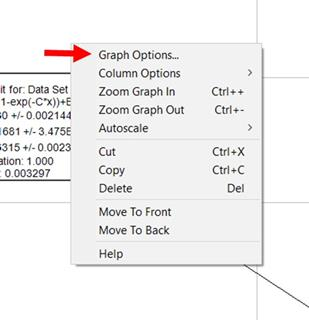
\includegraphics[width=2.6083in,height=2.7008in]{PH4CAX3M}
\end{figure}%
On the \textquotedblleft Graph Options\textquotedblright\ dialog make sure
both $x$ and $y$-error bars are checked.

\begin{figure}[h!]
	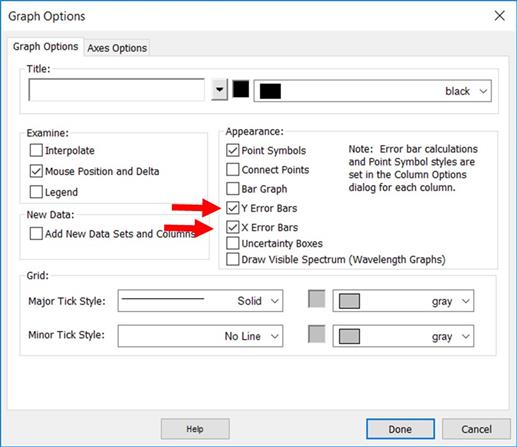
\includegraphics[width=4.3509in,height=3.7645in]{PH4CAX3N}
\end{figure}Chose \textquotedblleft
Done\textquotedblright\ and right click on the graph again. This time choose
\textquotedblleft Column Options.\textquotedblright\ \begin{figure}[h!]
	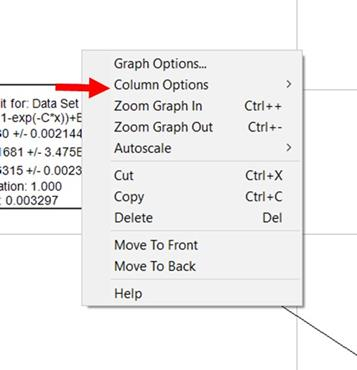
\includegraphics[width=3.0104in,height=%
	3.1185in]{PH4CAX3O}
\end{figure}and choose the $y$-data set.
Another dialog appears with two tabs. Choose the \textquotedblleft
Options\textquotedblright\ tab. \begin{figure}[h!]
	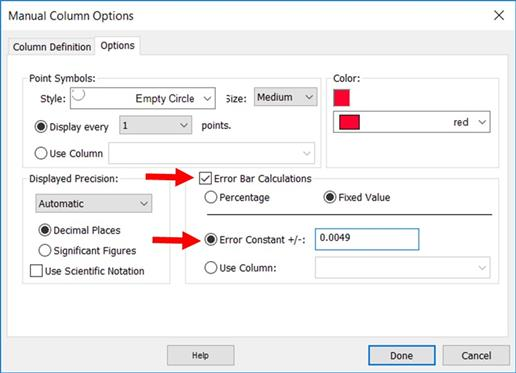
\includegraphics[width=4.3431in,height=3.1453in]{PH4CAX3P}
\end{figure}

You will see a place to choose how error bars are calculated. If you used
the simple voltmeter sketch as your basis, you know the quantization error
is about $4.9\unit{mV}.$ That will be true for every voltage measurement so
we can input this as a constant value. If you used a voltage divider, you
will have to use your calculated error value here. When you have your error
value in place, choose \textquotedblleft Done.\textquotedblright\ \begin{figure}[h!]
	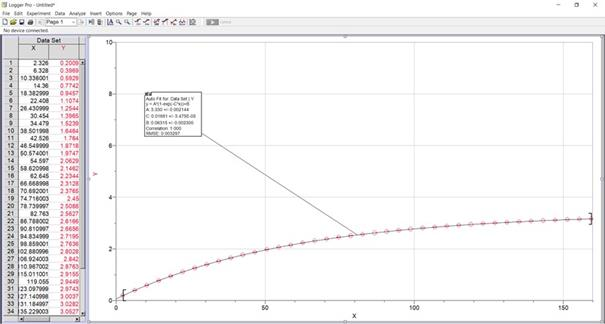
\includegraphics[width=5.0886in,height=2.7345in]{PH4CAX3Q}
\end{figure}

The voltage error was so small that it is hard to see the error bars! That
is fine. What this tells us is that our fit line must go right through the
center of each data point. But it does. So we are really doing fine. The
data supports the model.

But now let's go back to our little box of curve fit parameters. We
identified 
\begin{equation*}
	\tau =\frac{1}{\mathtt{C}}
\end{equation*}%
and for my data I have 
\begin{equation*}
	\mathtt{C}=0.01681\pm 3.475\times 10^{-5}
\end{equation*}%
\newline
We need units, and looking at the equation we know $\tau $ has units of
seconds, so $\mathtt{C}$ must have units of inverse seconds.%
\begin{equation*}
	\mathtt{C}=\left( 0.01681\pm 3.475\times 10^{-5}\right) \frac{1}{\unit{s}}
\end{equation*}%
so we can find a value for $\tau .$ For my data, I have 
\begin{eqnarray*}
	\tau _{measured} &=&\frac{1}{0.01681\frac{1}{\unit{s}}} \\
	&=&59.\,\allowbreak 488\unit{s}
\end{eqnarray*}

Note that we will have to calculate the uncertainty in $\tau .$ I will leave
that for an exercise. But I can compare this $\tau _{measured}$ to the $\tau
=RC$ value I started with. If they are within each other's error range, this
is a powerful confirmation of our capacitor model.

%TCIMACRO{\TeXButton{\vspace*{\fill}}{\vspace*{\fill}}}%
%BeginExpansion
\vspace*{\fill}%
%EndExpansion
\pagebreak